% Appendix
\appendix

\chapter{Παρουσίαση διεπαφής \emph{RASA-X}}
\label{chapter:appendix}
Στο παρόν παράρτημα παρουσιάζονται μερικά από τα κύρια σημεία της δικτυακής διεπαφής \emph{RASA-X}. Μέσω της διεπαφής παρέχεται η δυνατότητα τροποποίησης όλων των αρχείων που χρησιμοποιούνται για την εκπαίδευση του ψηφιακού βοηθού, σχήματα \ref{fig:rasax-config}, \ref{fig:rasax-domain}, \ref{fig:rasax-training}, \ref{fig:rasax-stories}, \ref{fig:rasax-rules}, \ref{fig:rasax-responses} αλλά και η δυνατότητα επανεκπαίδευσης του. Τέλος, στα σχήματα \ref{fig:rasax-conversation-interactive}, \ref{fig:rasax-conversation-review} παρουσιάζονται τα εργαλεία για διαδραστική συζήτηση με τον ψηφιακό βοηθό και η αξιολόγηση υπαρχουσών συζητήσεων αντίστοιχα.

\begin{figure}[!ht]
  \centering
  \captionsetup{justification=centering}
  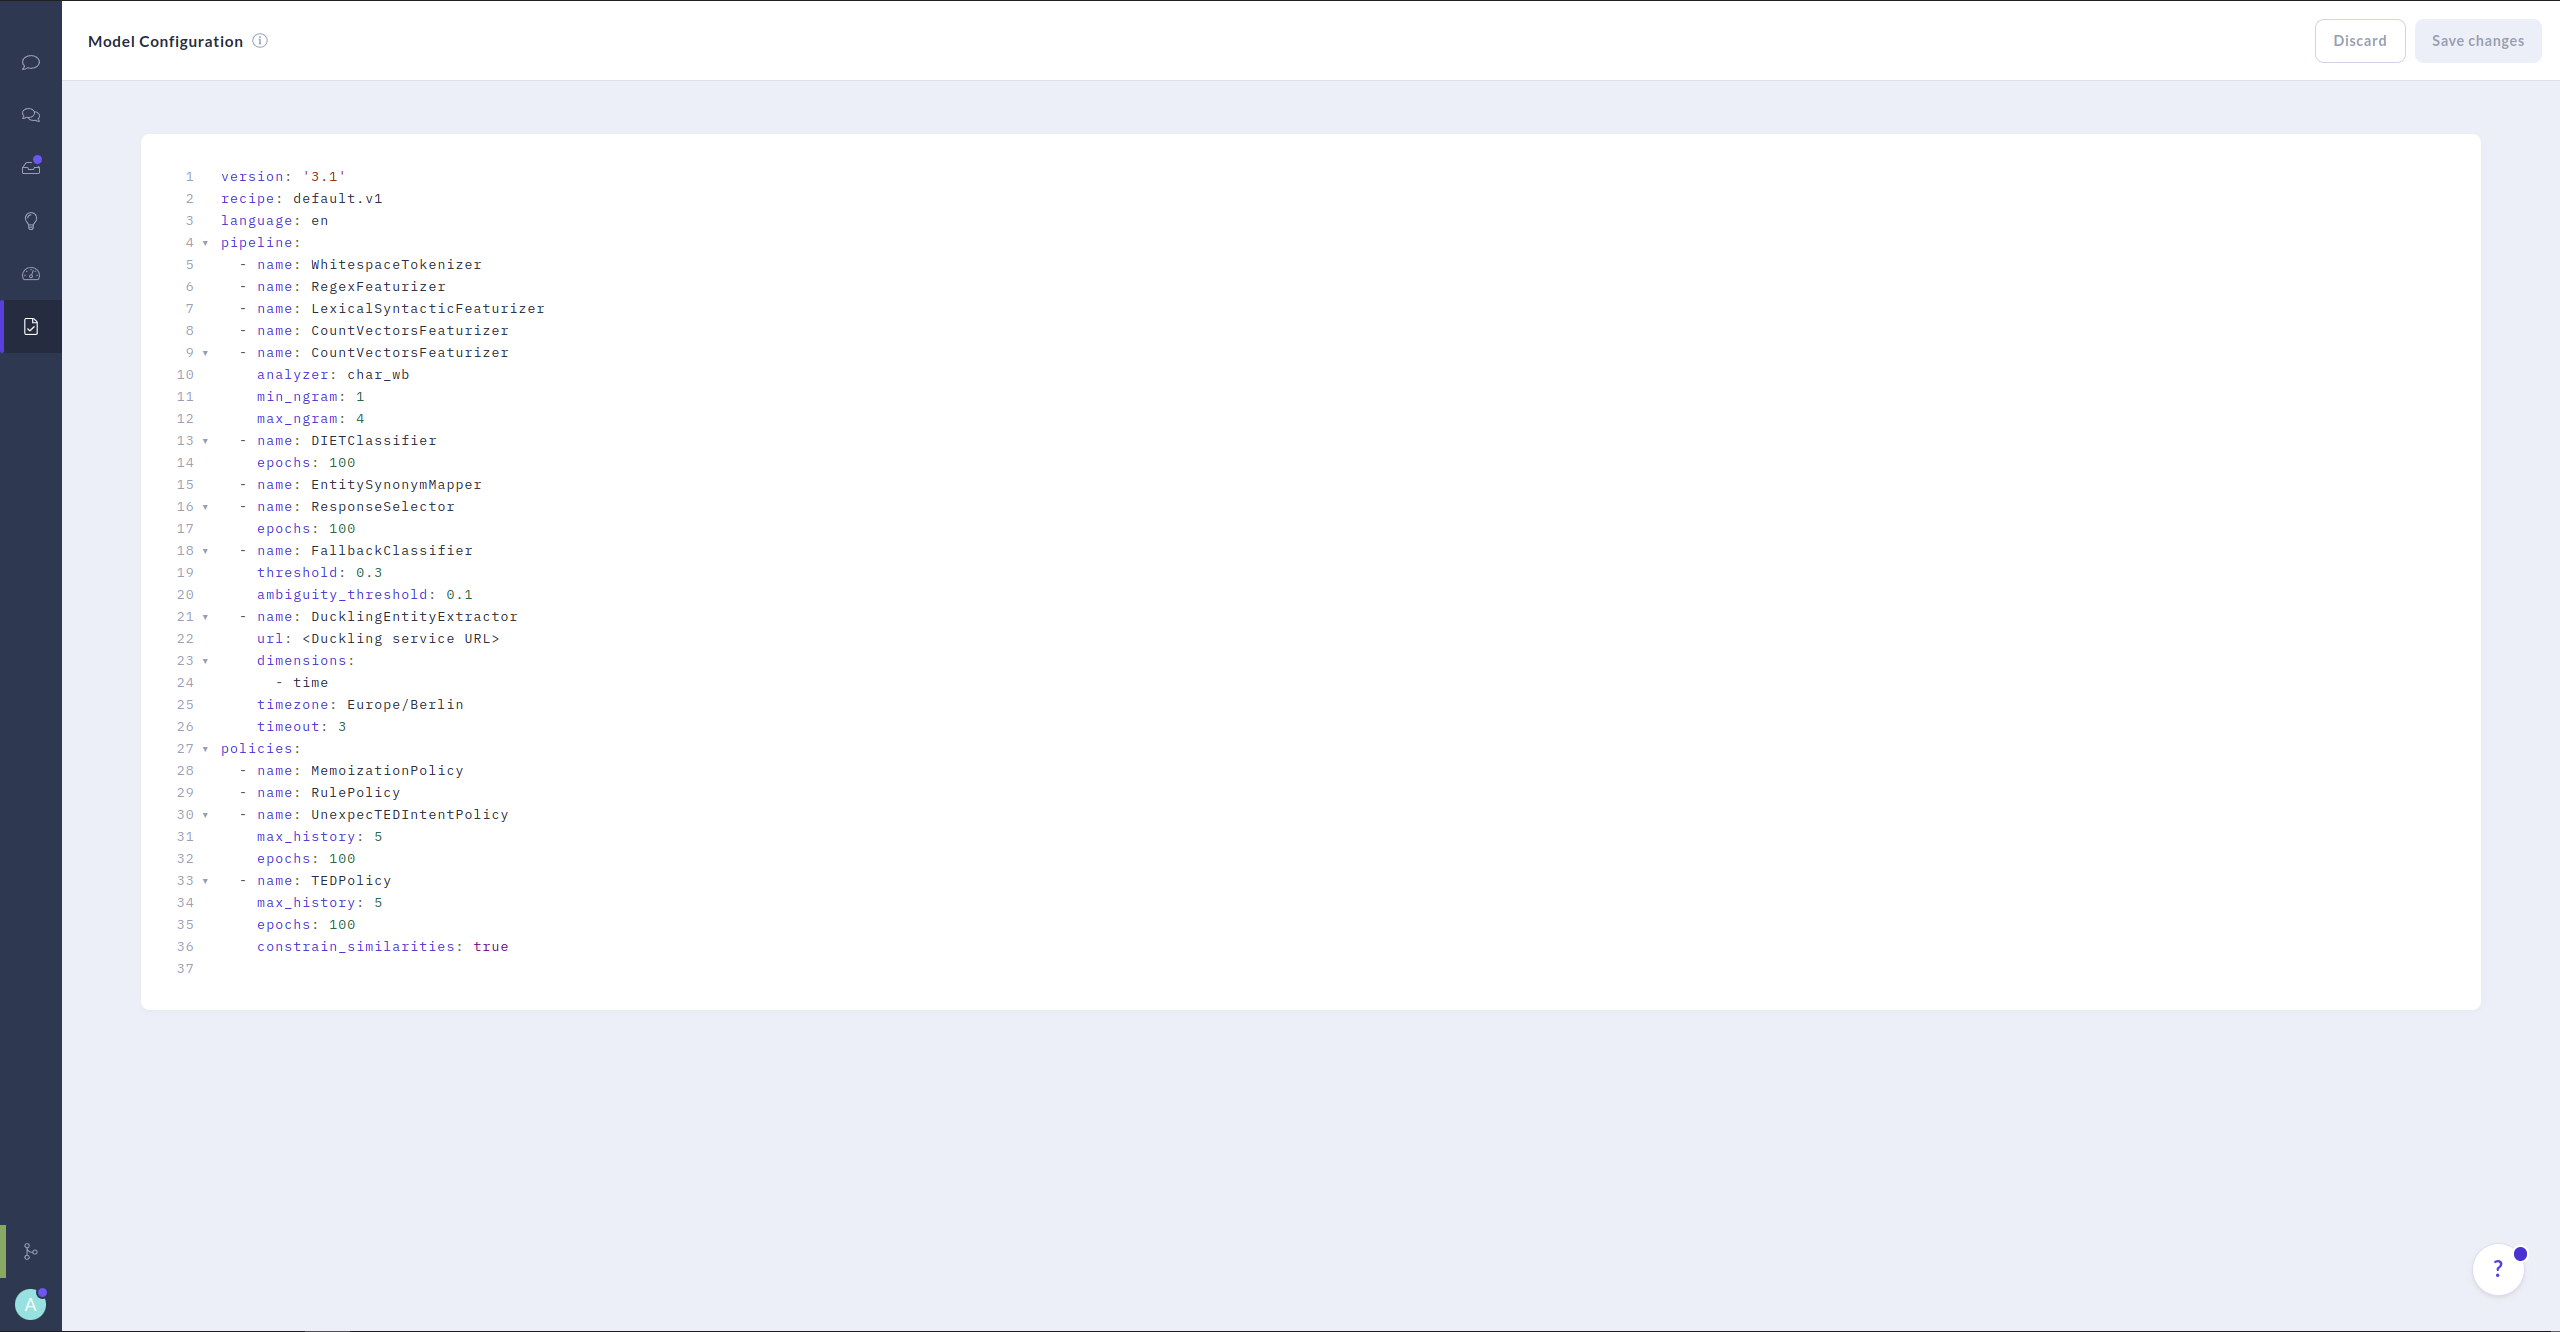
\includegraphics[width=1\textwidth]{images/appendix/rasax-config.png}
  \caption{\emph{RASA-X} αρχείο \emph{config}}
  \label{fig:rasax-config}
\end{figure}
\noindent

\begin{figure}[!ht]
  \centering
  \captionsetup{justification=centering}
  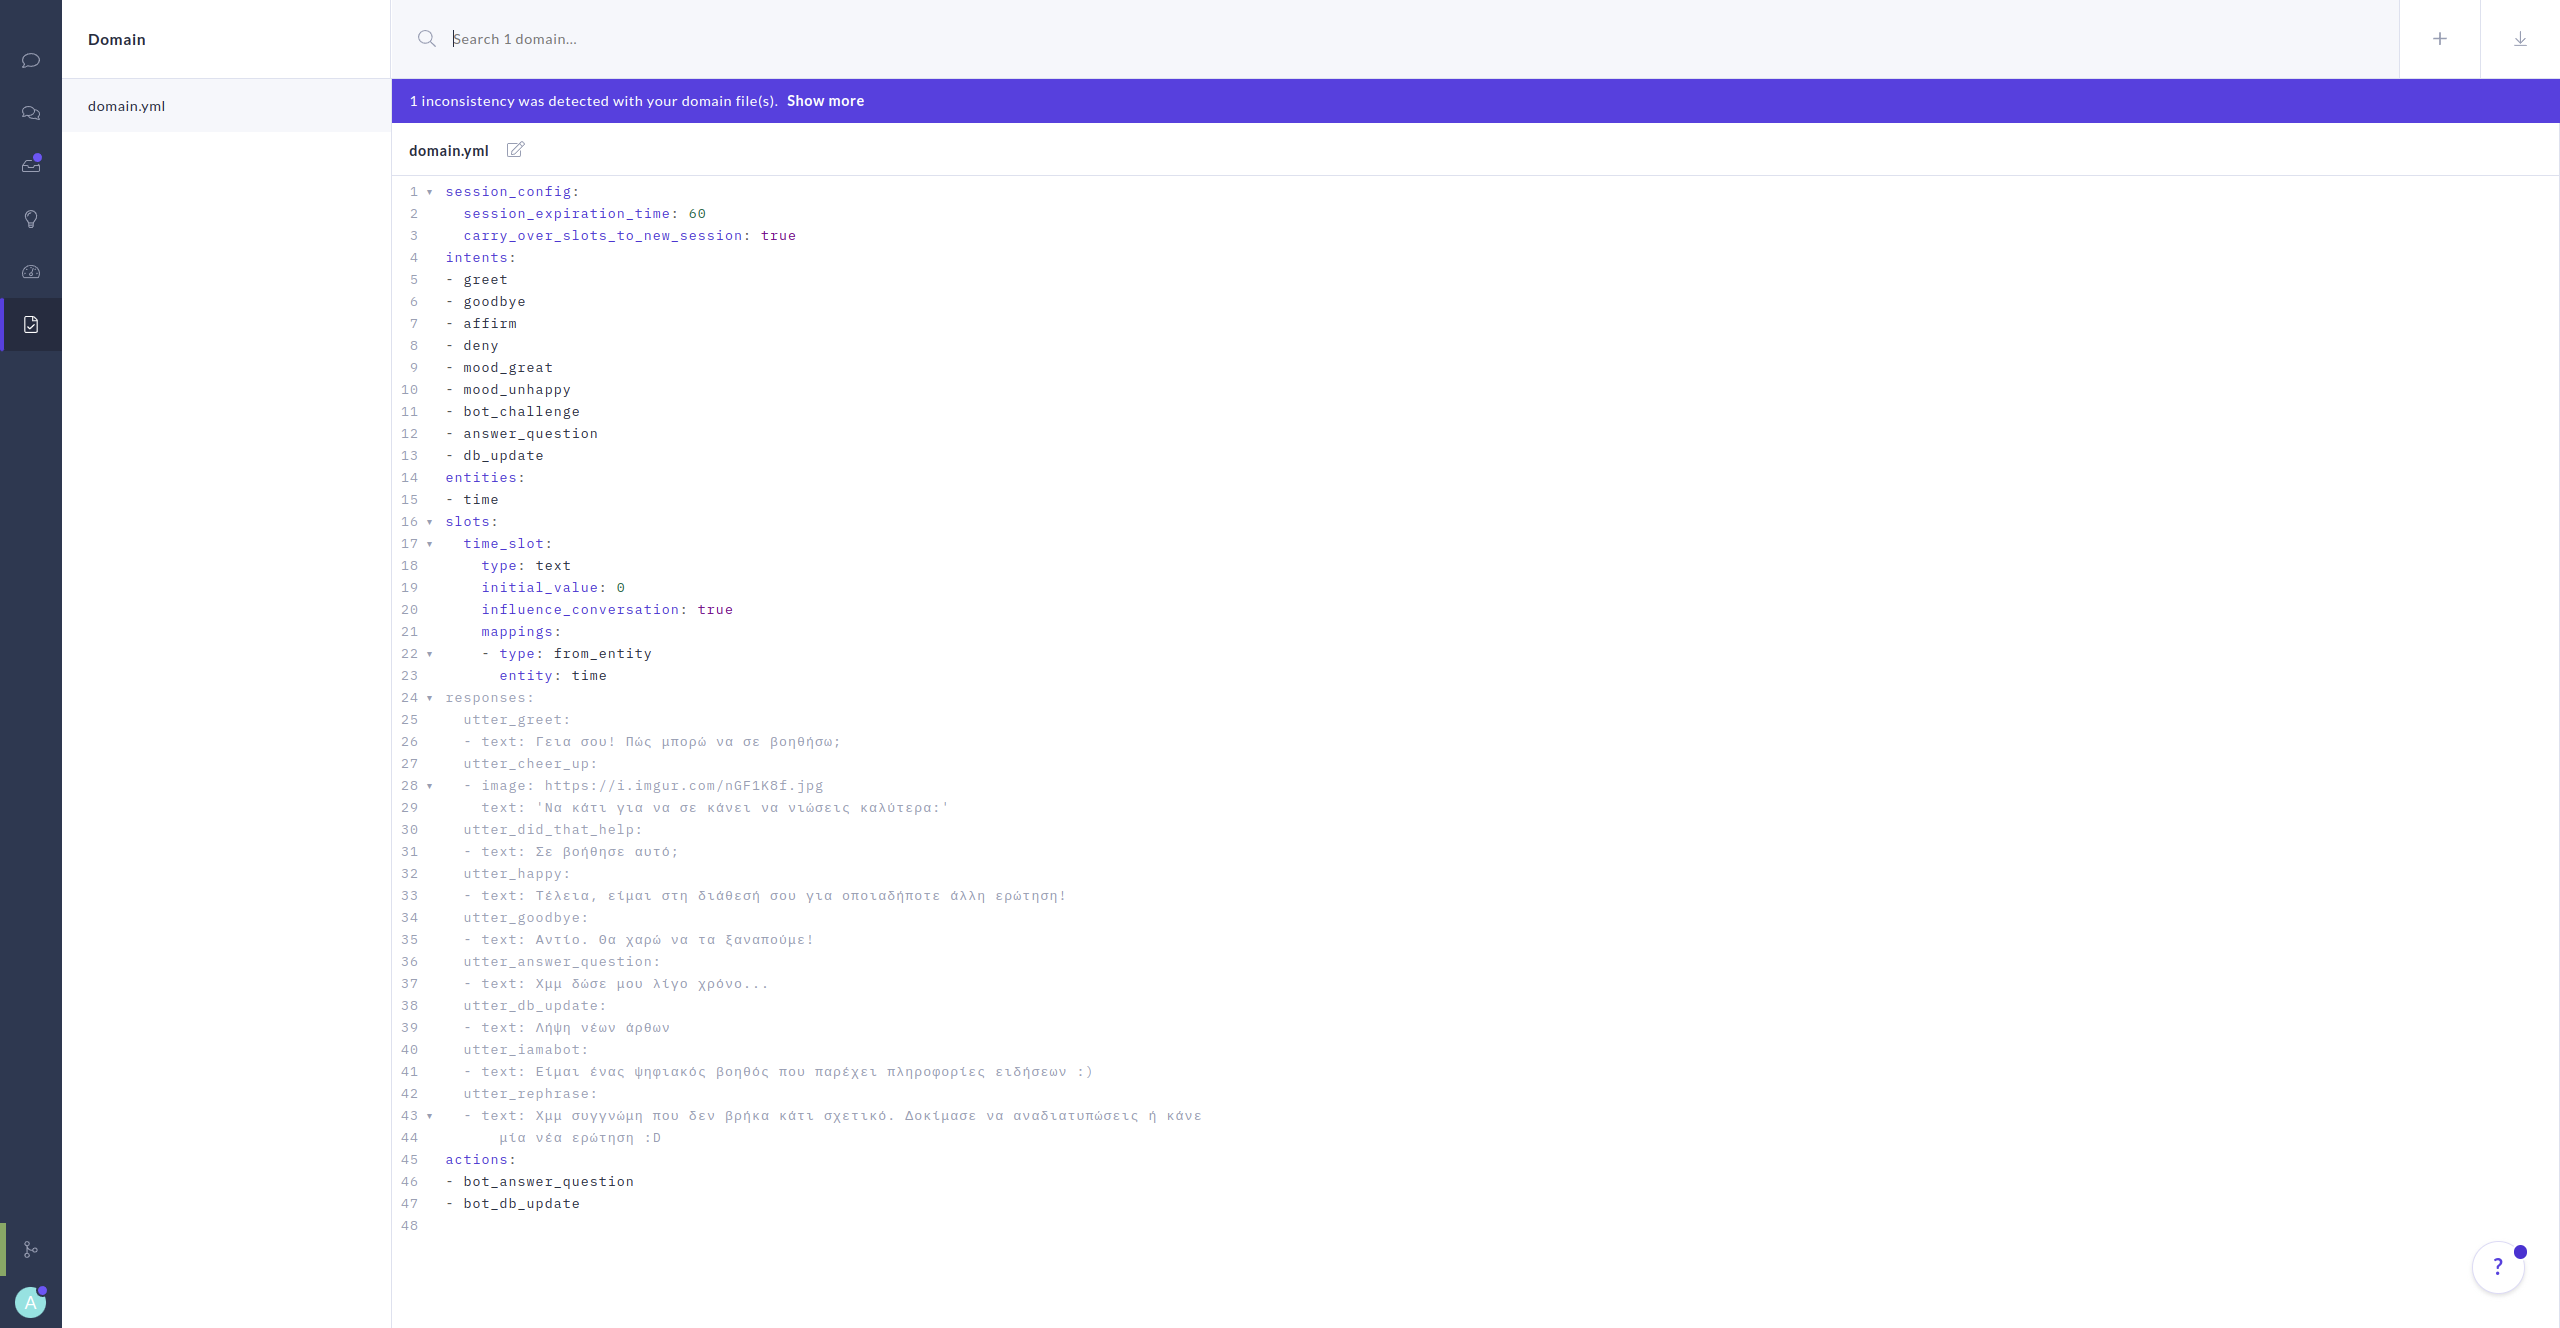
\includegraphics[width=1\textwidth]{images/appendix/rasax-domain.png}
  \caption{\emph{RASA-X} αρχείο \emph{domain}}
  \label{fig:rasax-domain}
\end{figure}
\noindent

\begin{figure}[!ht]
  \centering
  \captionsetup{justification=centering}
  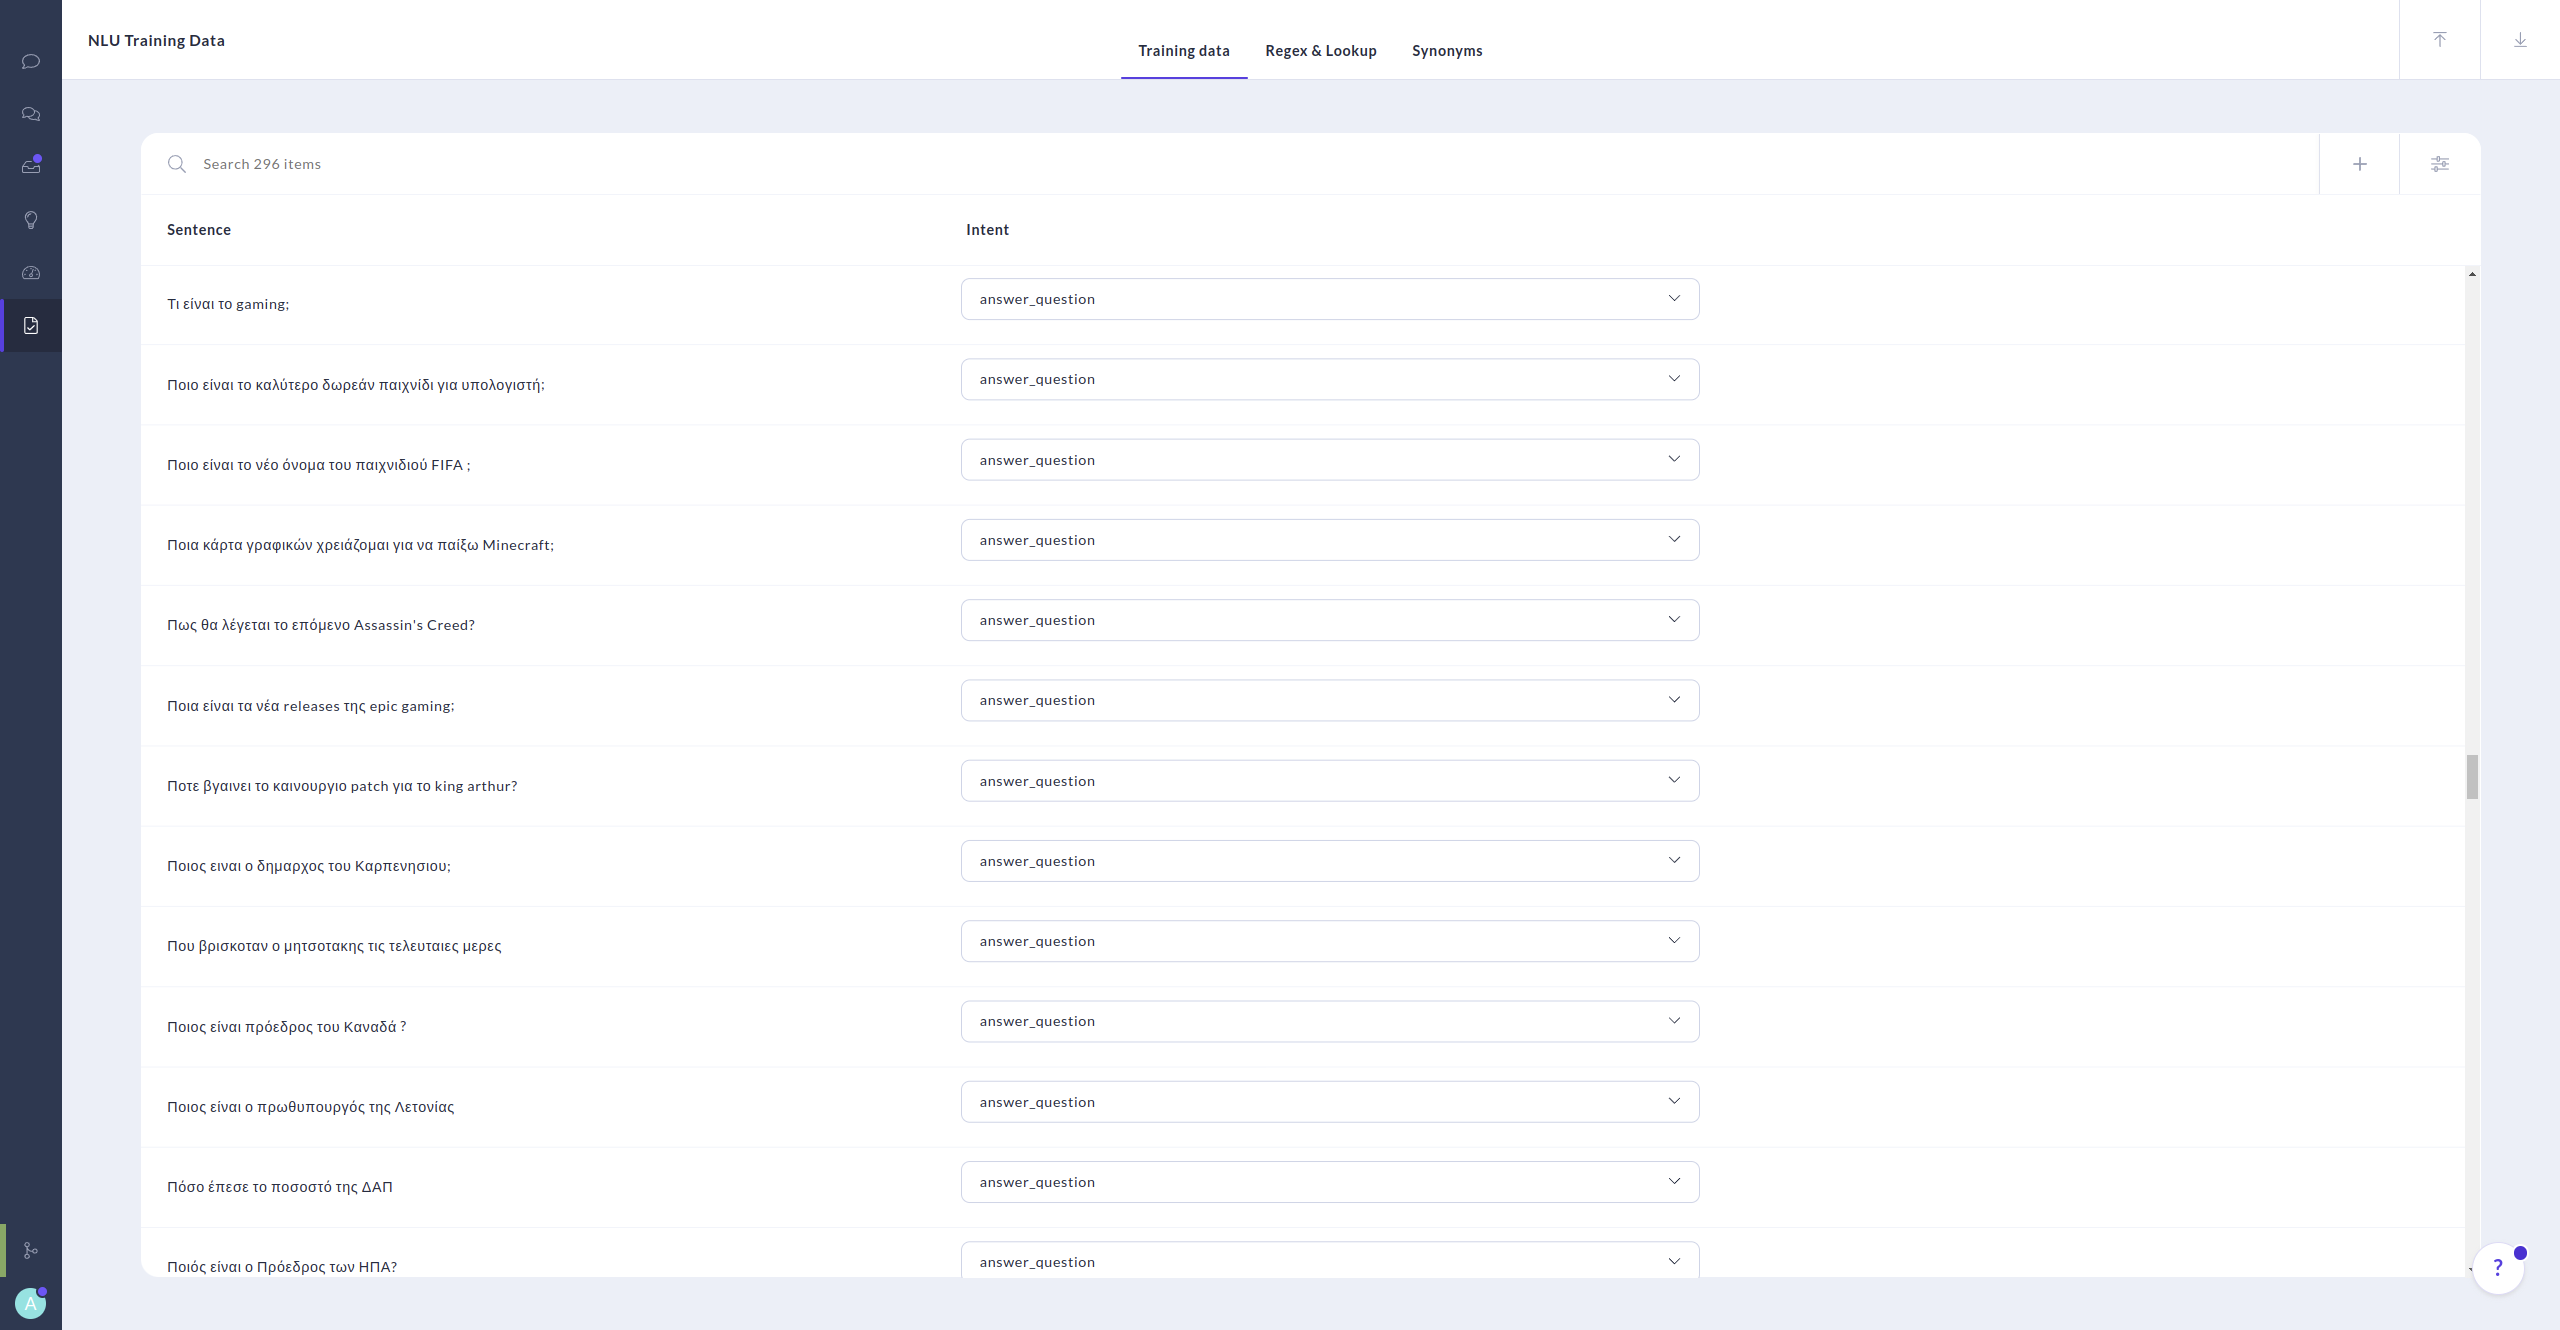
\includegraphics[width=1\textwidth]{images/appendix/rasax-training.png}
  \caption{\emph{RASA-X} αρχείο με δεδομένα εκπαίδευσης}
  \label{fig:rasax-training}
\end{figure}
\noindent

\begin{figure}[!ht]
  \centering
  \captionsetup{justification=centering}
  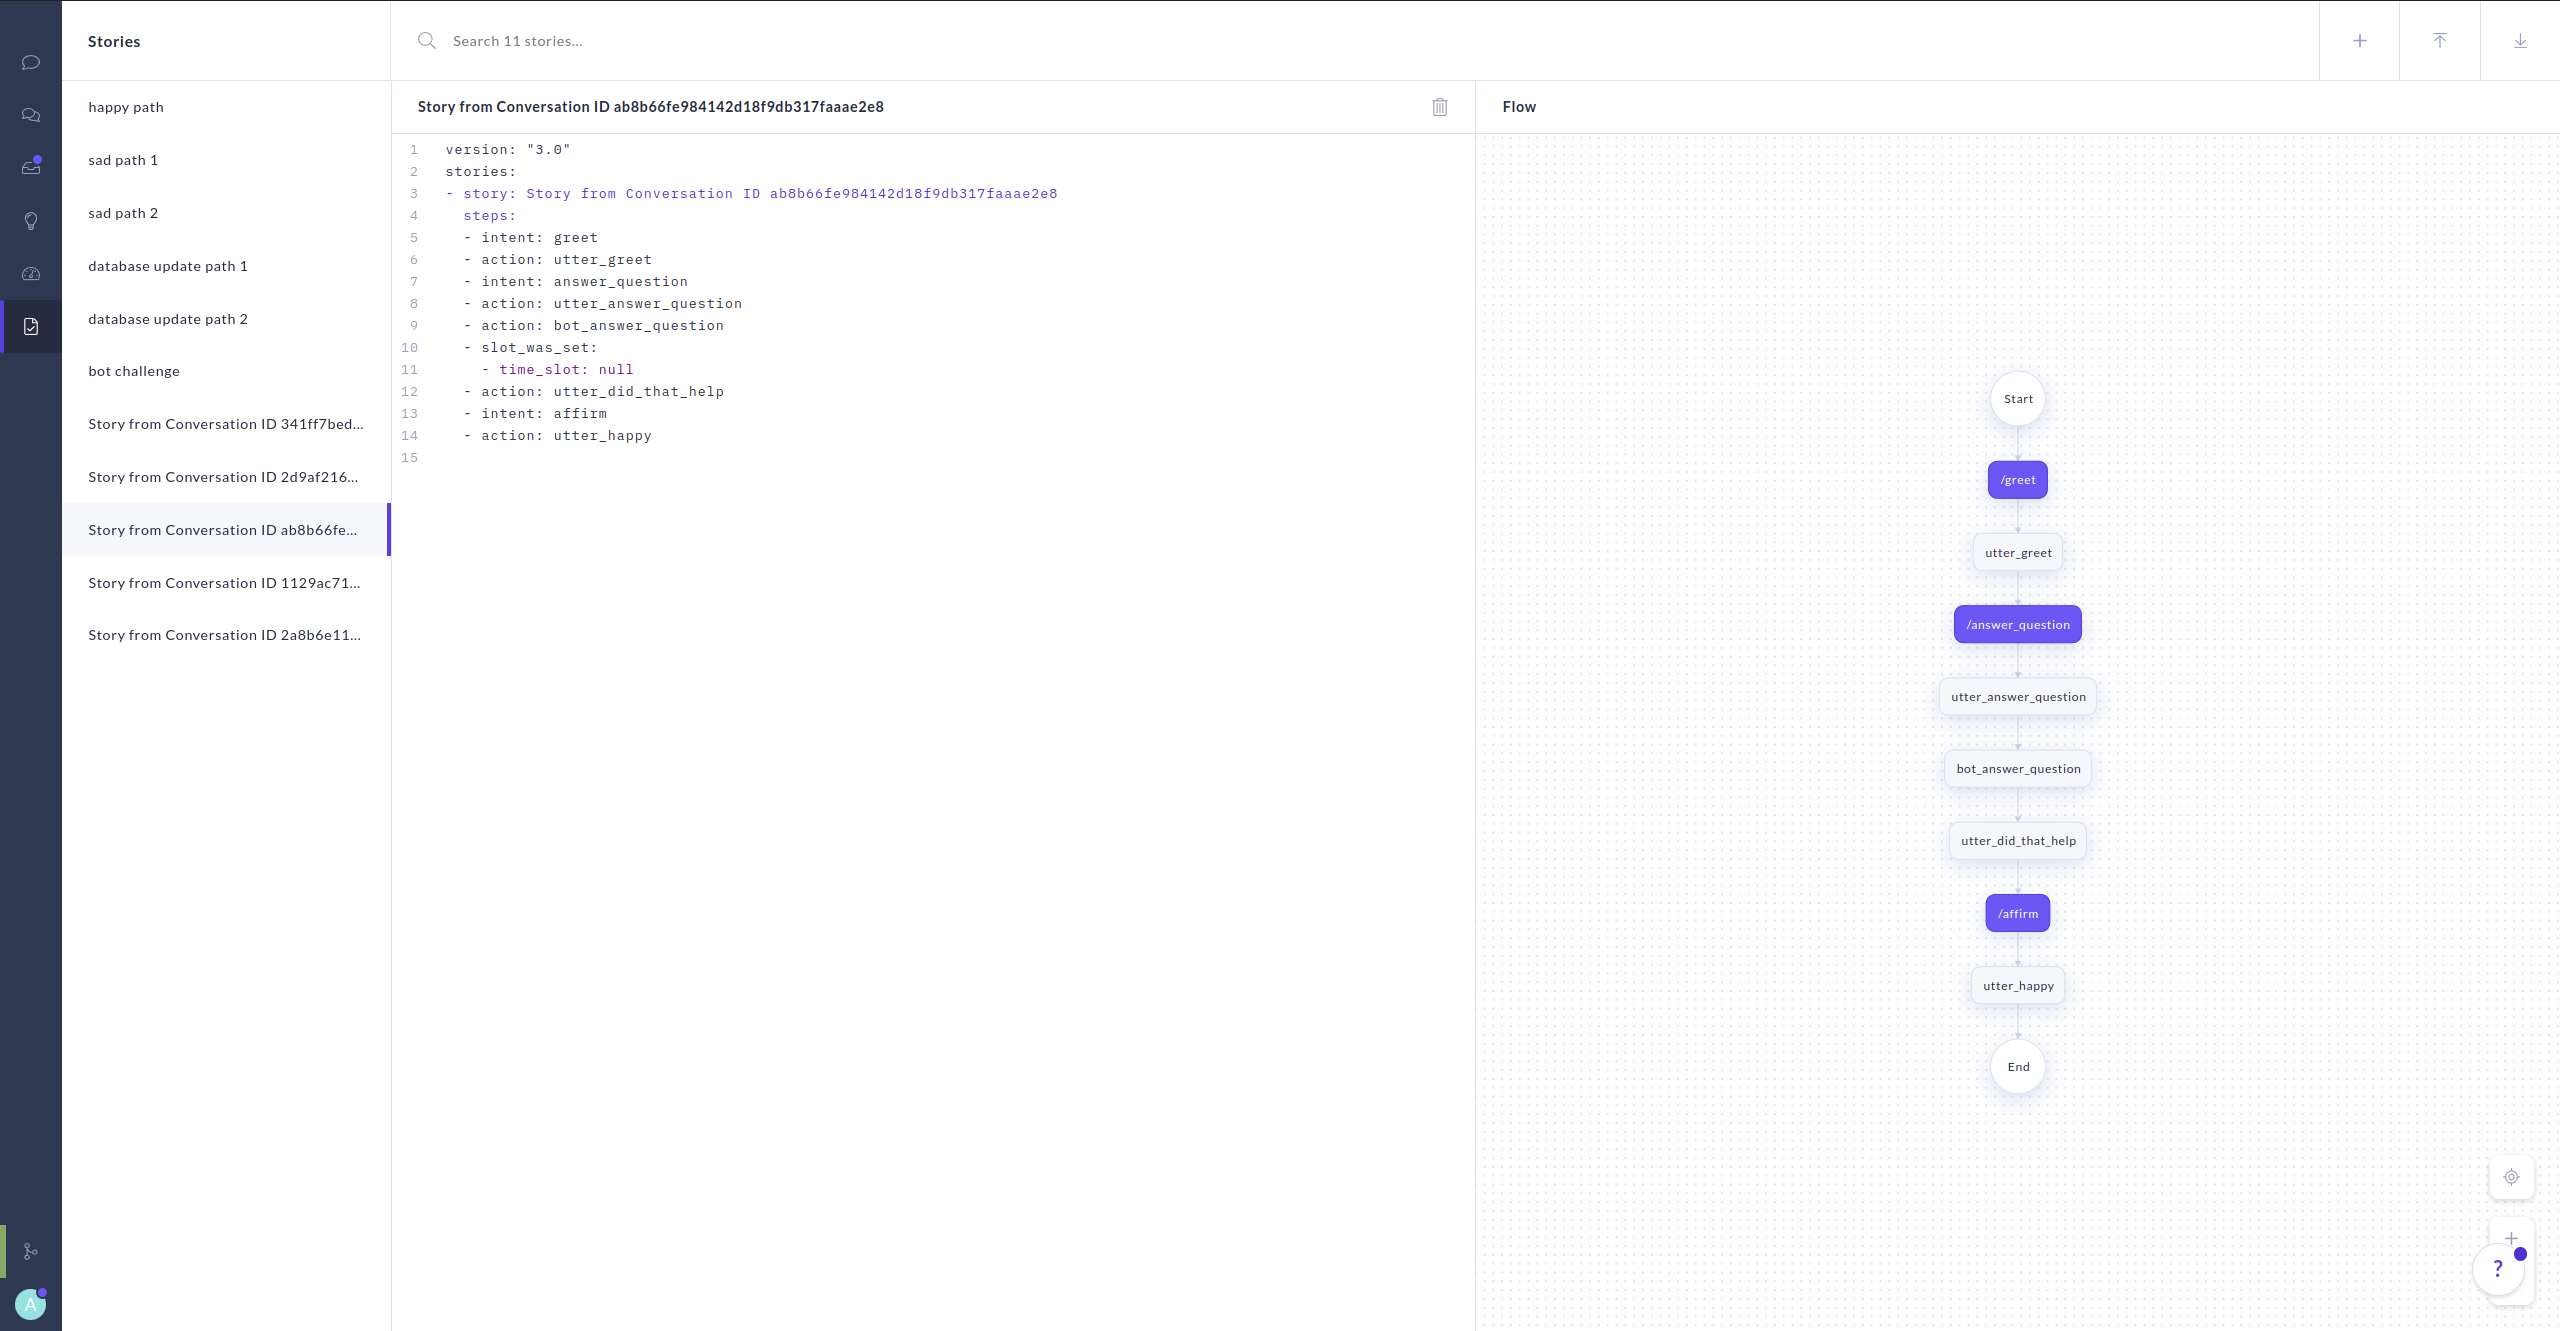
\includegraphics[width=1\textwidth]{images/appendix/rasax-stories.png}
  \caption{\emph{RASA-X} αρχείο με τις ιστορίες}
  \label{fig:rasax-stories}
\end{figure}
\noindent

\begin{figure}[!ht]
  \centering
  \captionsetup{justification=centering}
  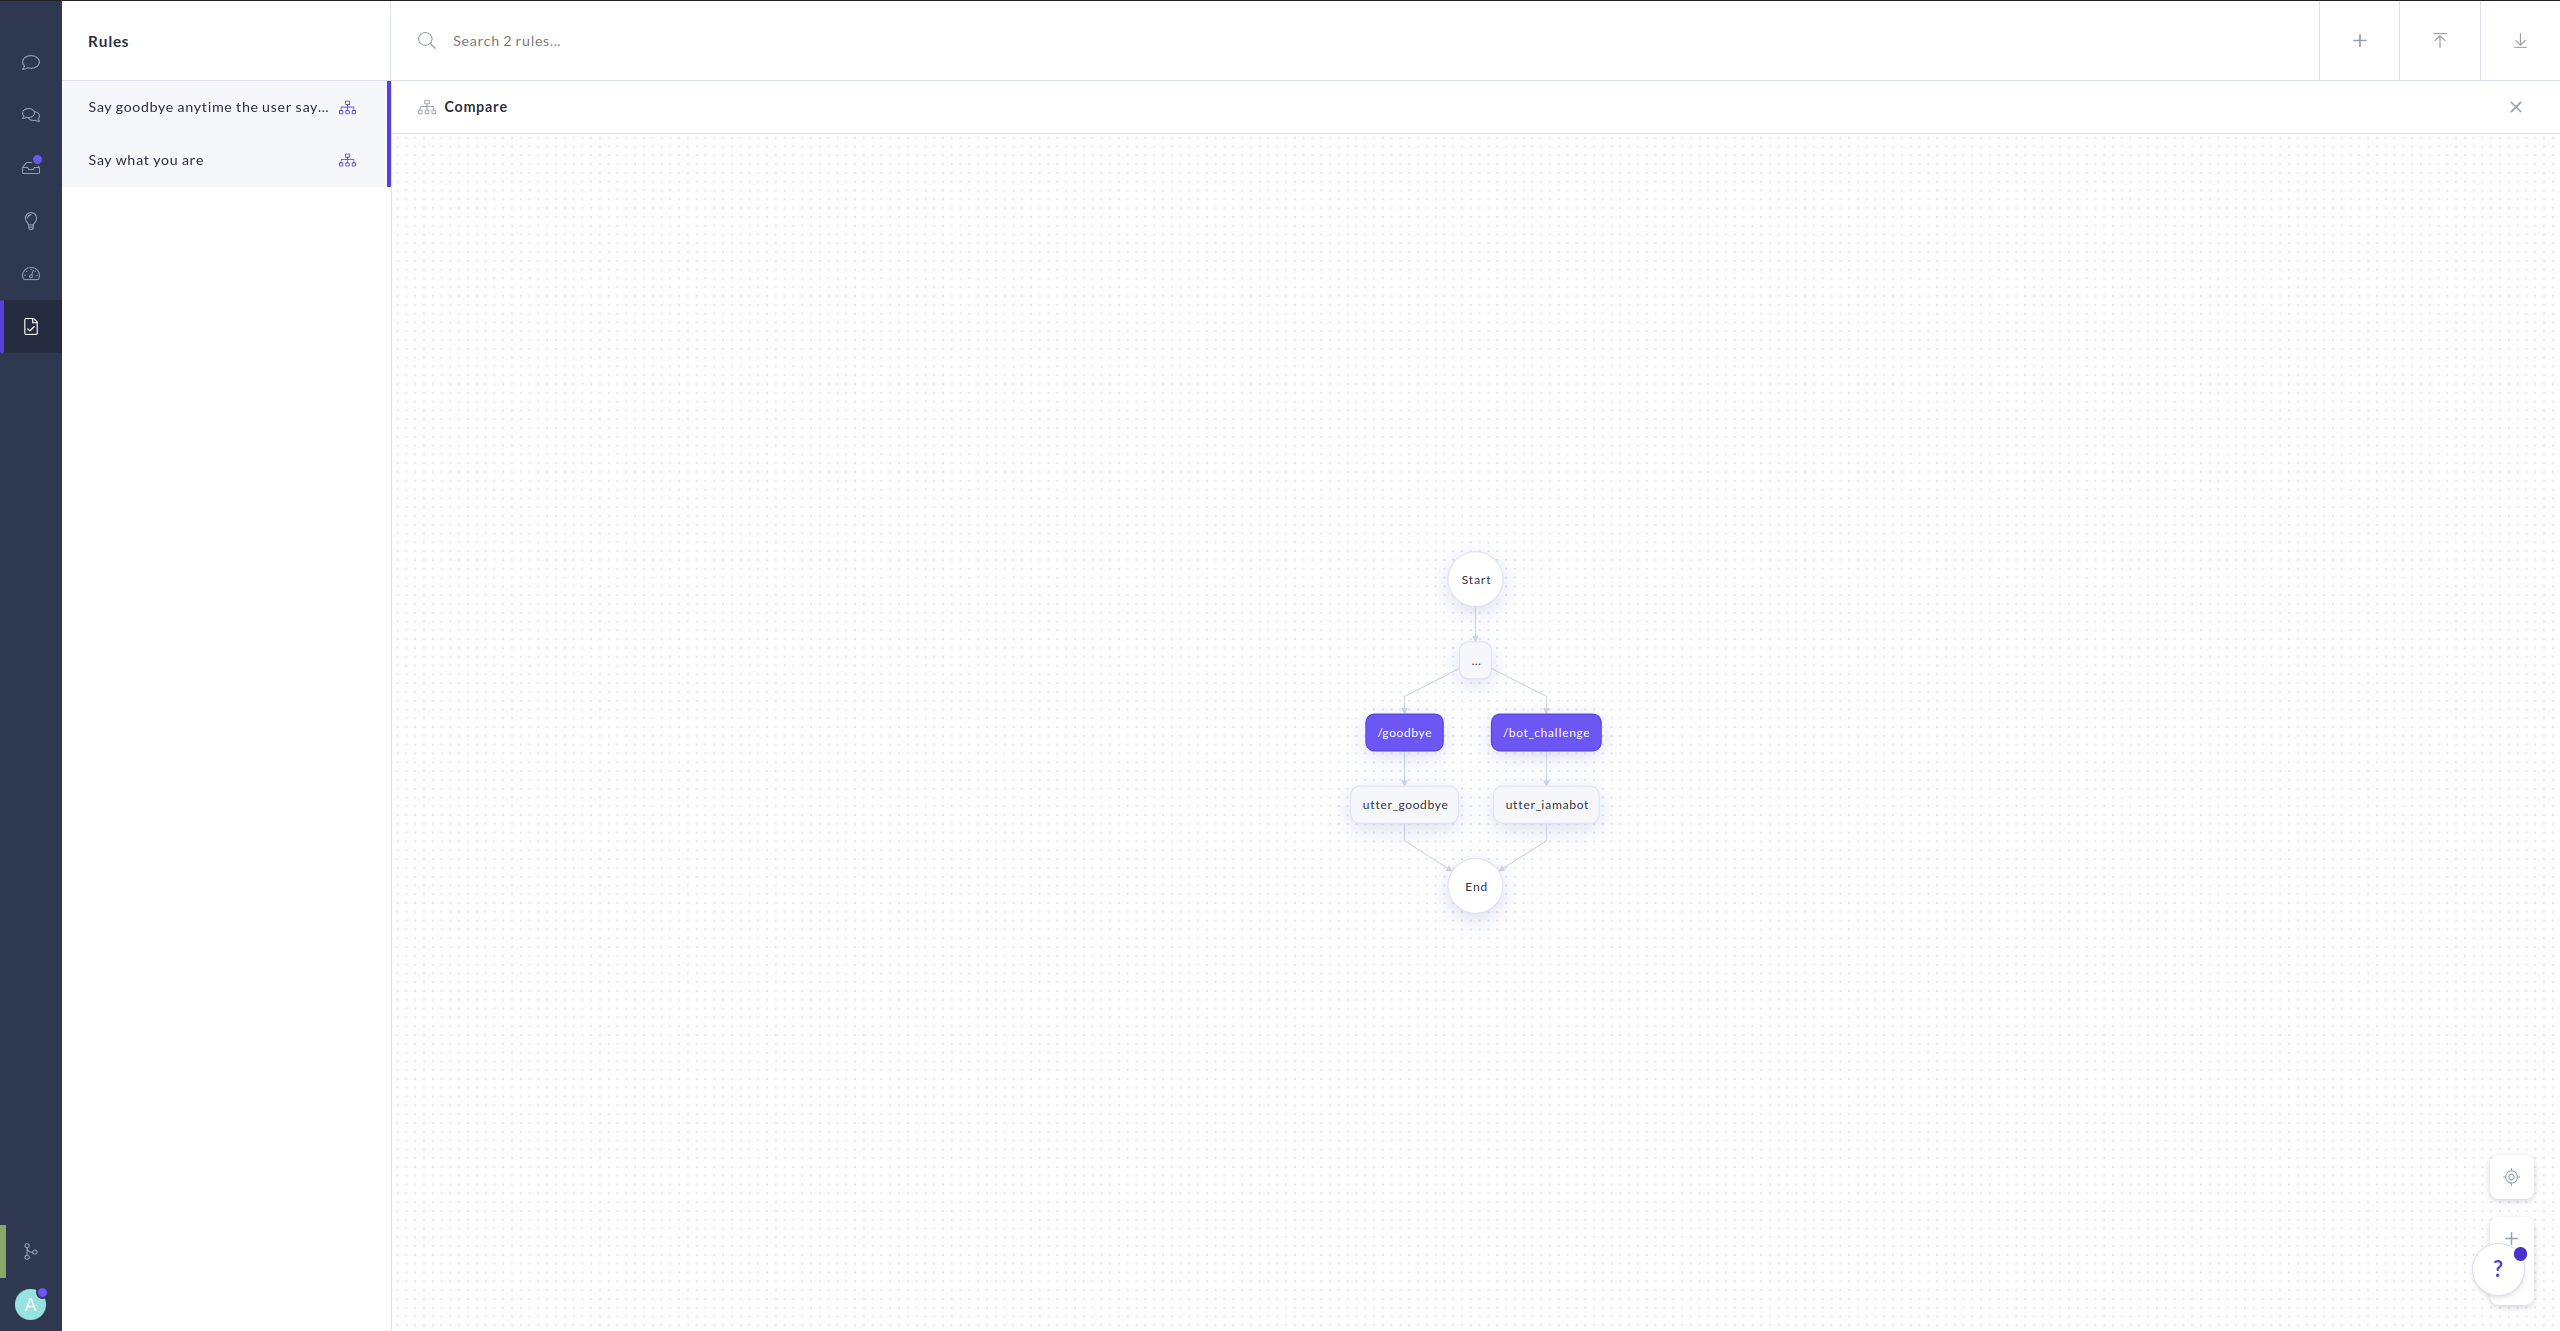
\includegraphics[width=1\textwidth]{images/appendix/rasax-rules.png}
  \caption{\emph{RASA-X} αρχείο με τους κανόνες}
  \label{fig:rasax-rules}
\end{figure}
\noindent

\begin{figure}[!ht]
  \centering
  \captionsetup{justification=centering}
  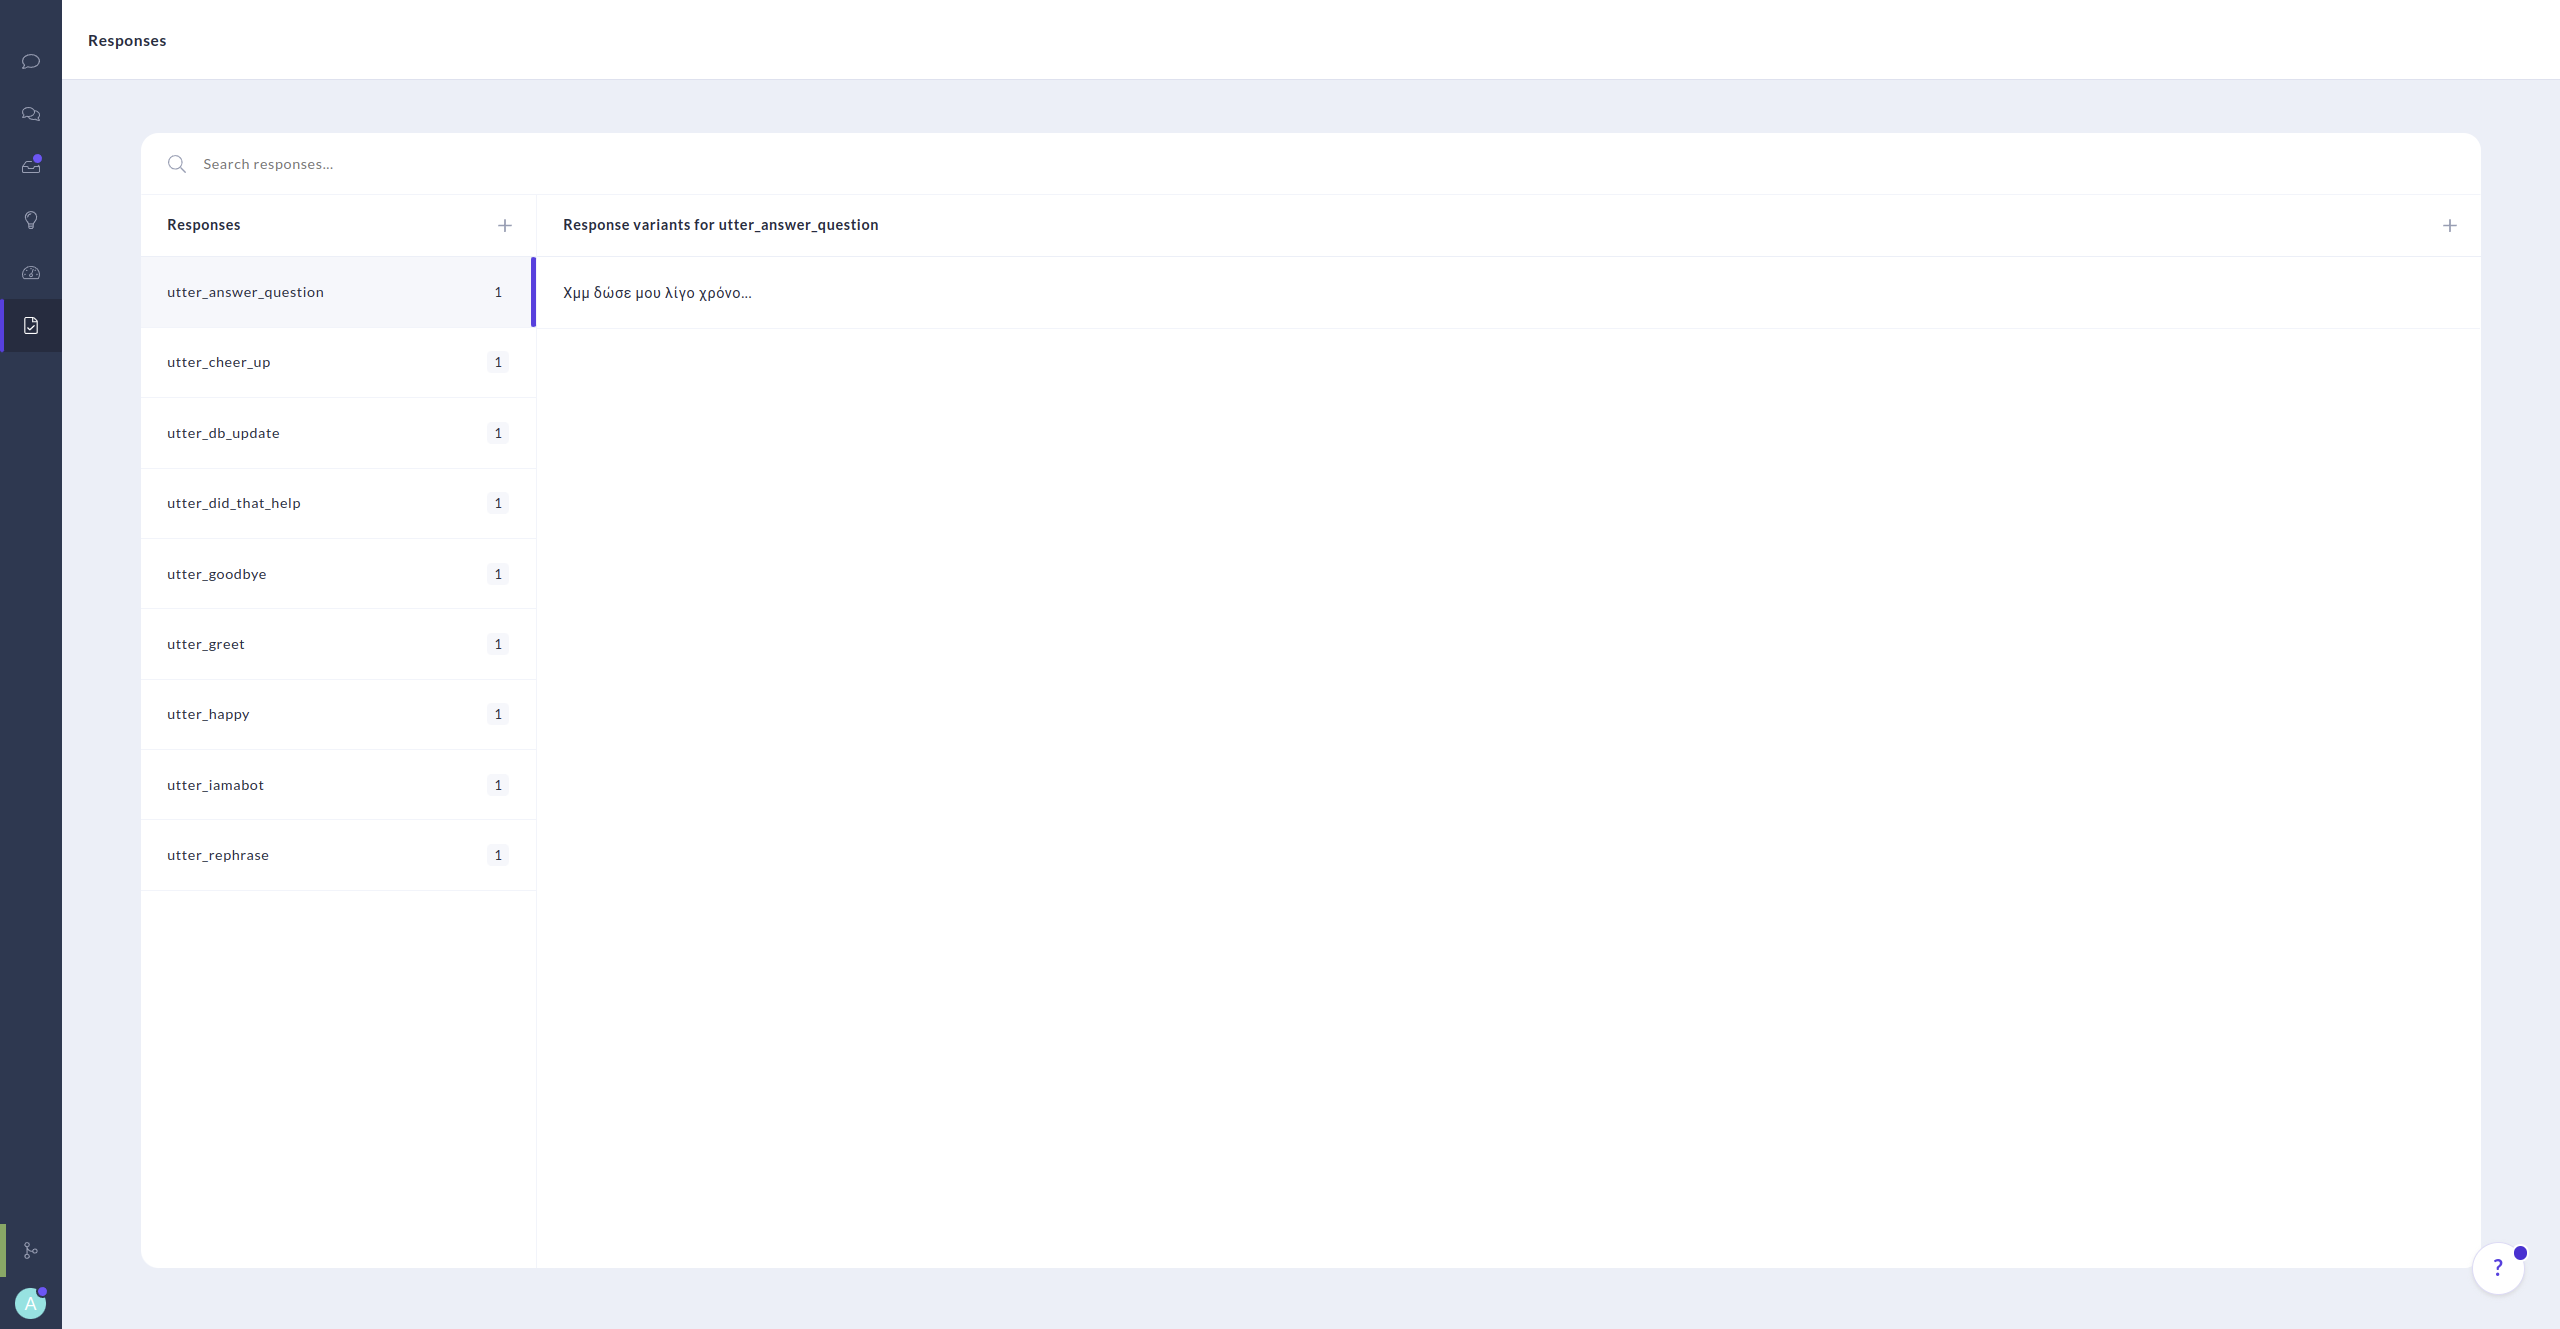
\includegraphics[width=1\textwidth]{images/appendix/rasax-responses.png}
  \caption{\emph{RASA-X} αρχείο με επιθυμίες χρήστη}
  \label{fig:rasax-responses}
\end{figure}
\noindent

\begin{figure}[!ht]
  \centering
  \captionsetup{justification=centering}
  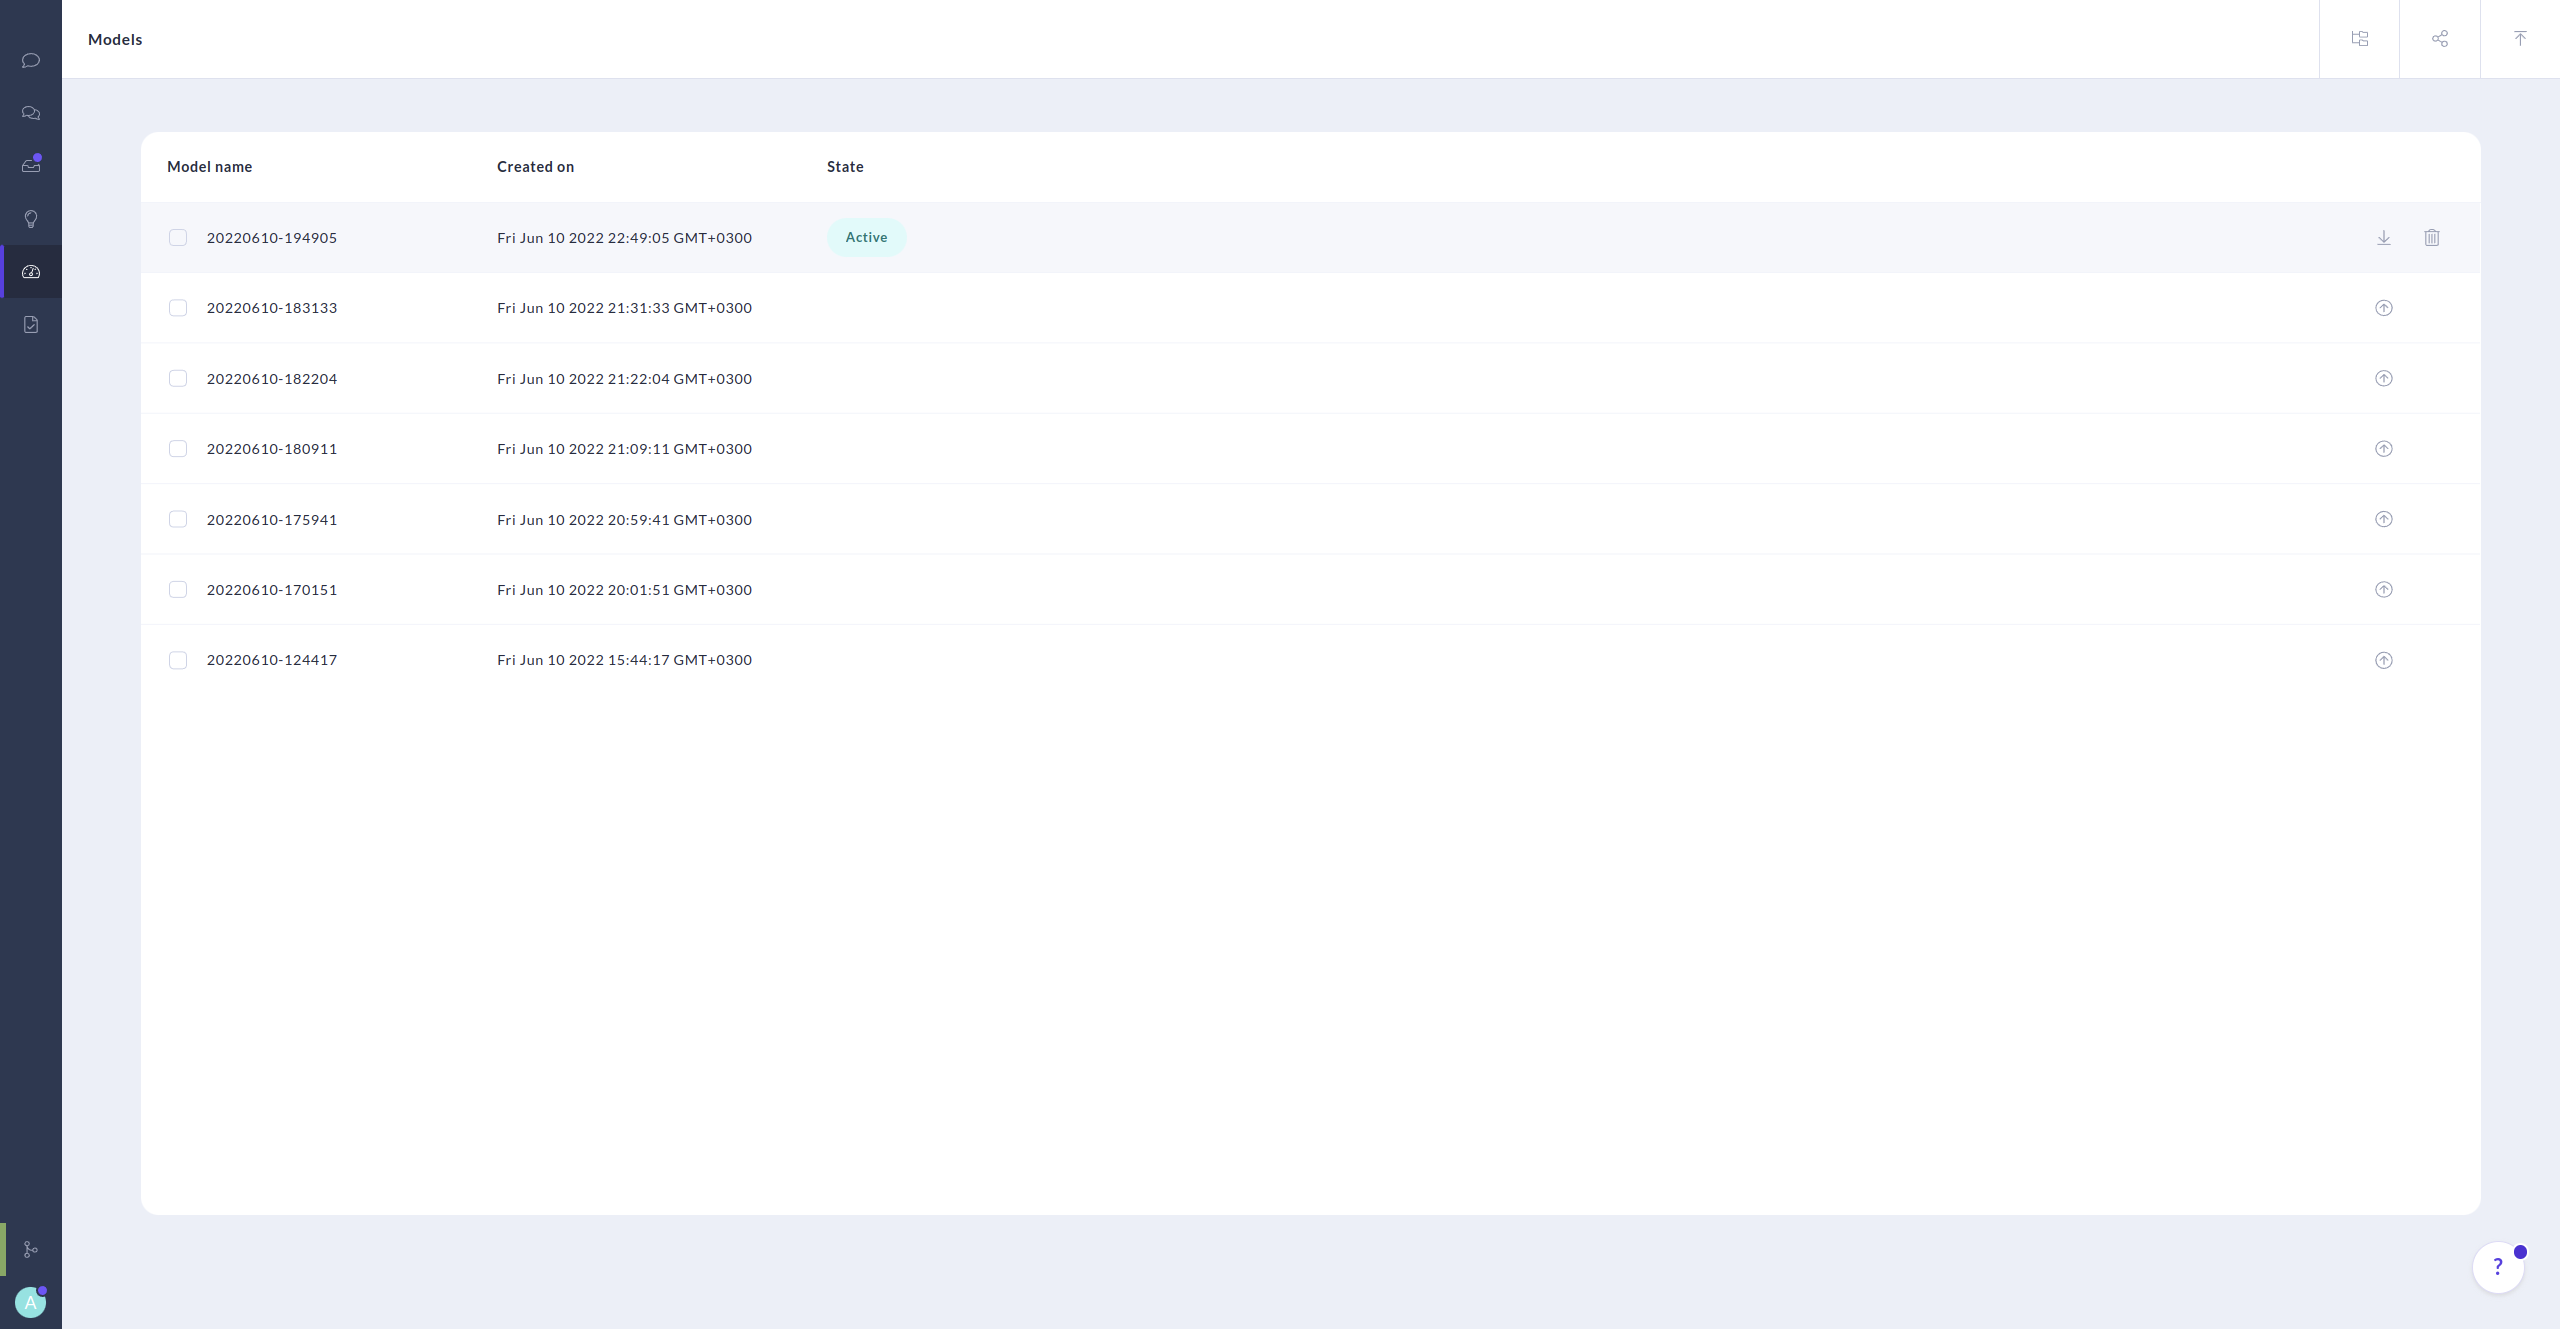
\includegraphics[width=1\textwidth]{images/appendix/rasax-models.png}
  \caption{\emph{RASA-X} εκπαιδευμένα μοντέλα}
  \label{fig:rasax-models}
\end{figure}
\noindent

\begin{figure}[!ht]
  \centering
  \captionsetup{justification=centering}
  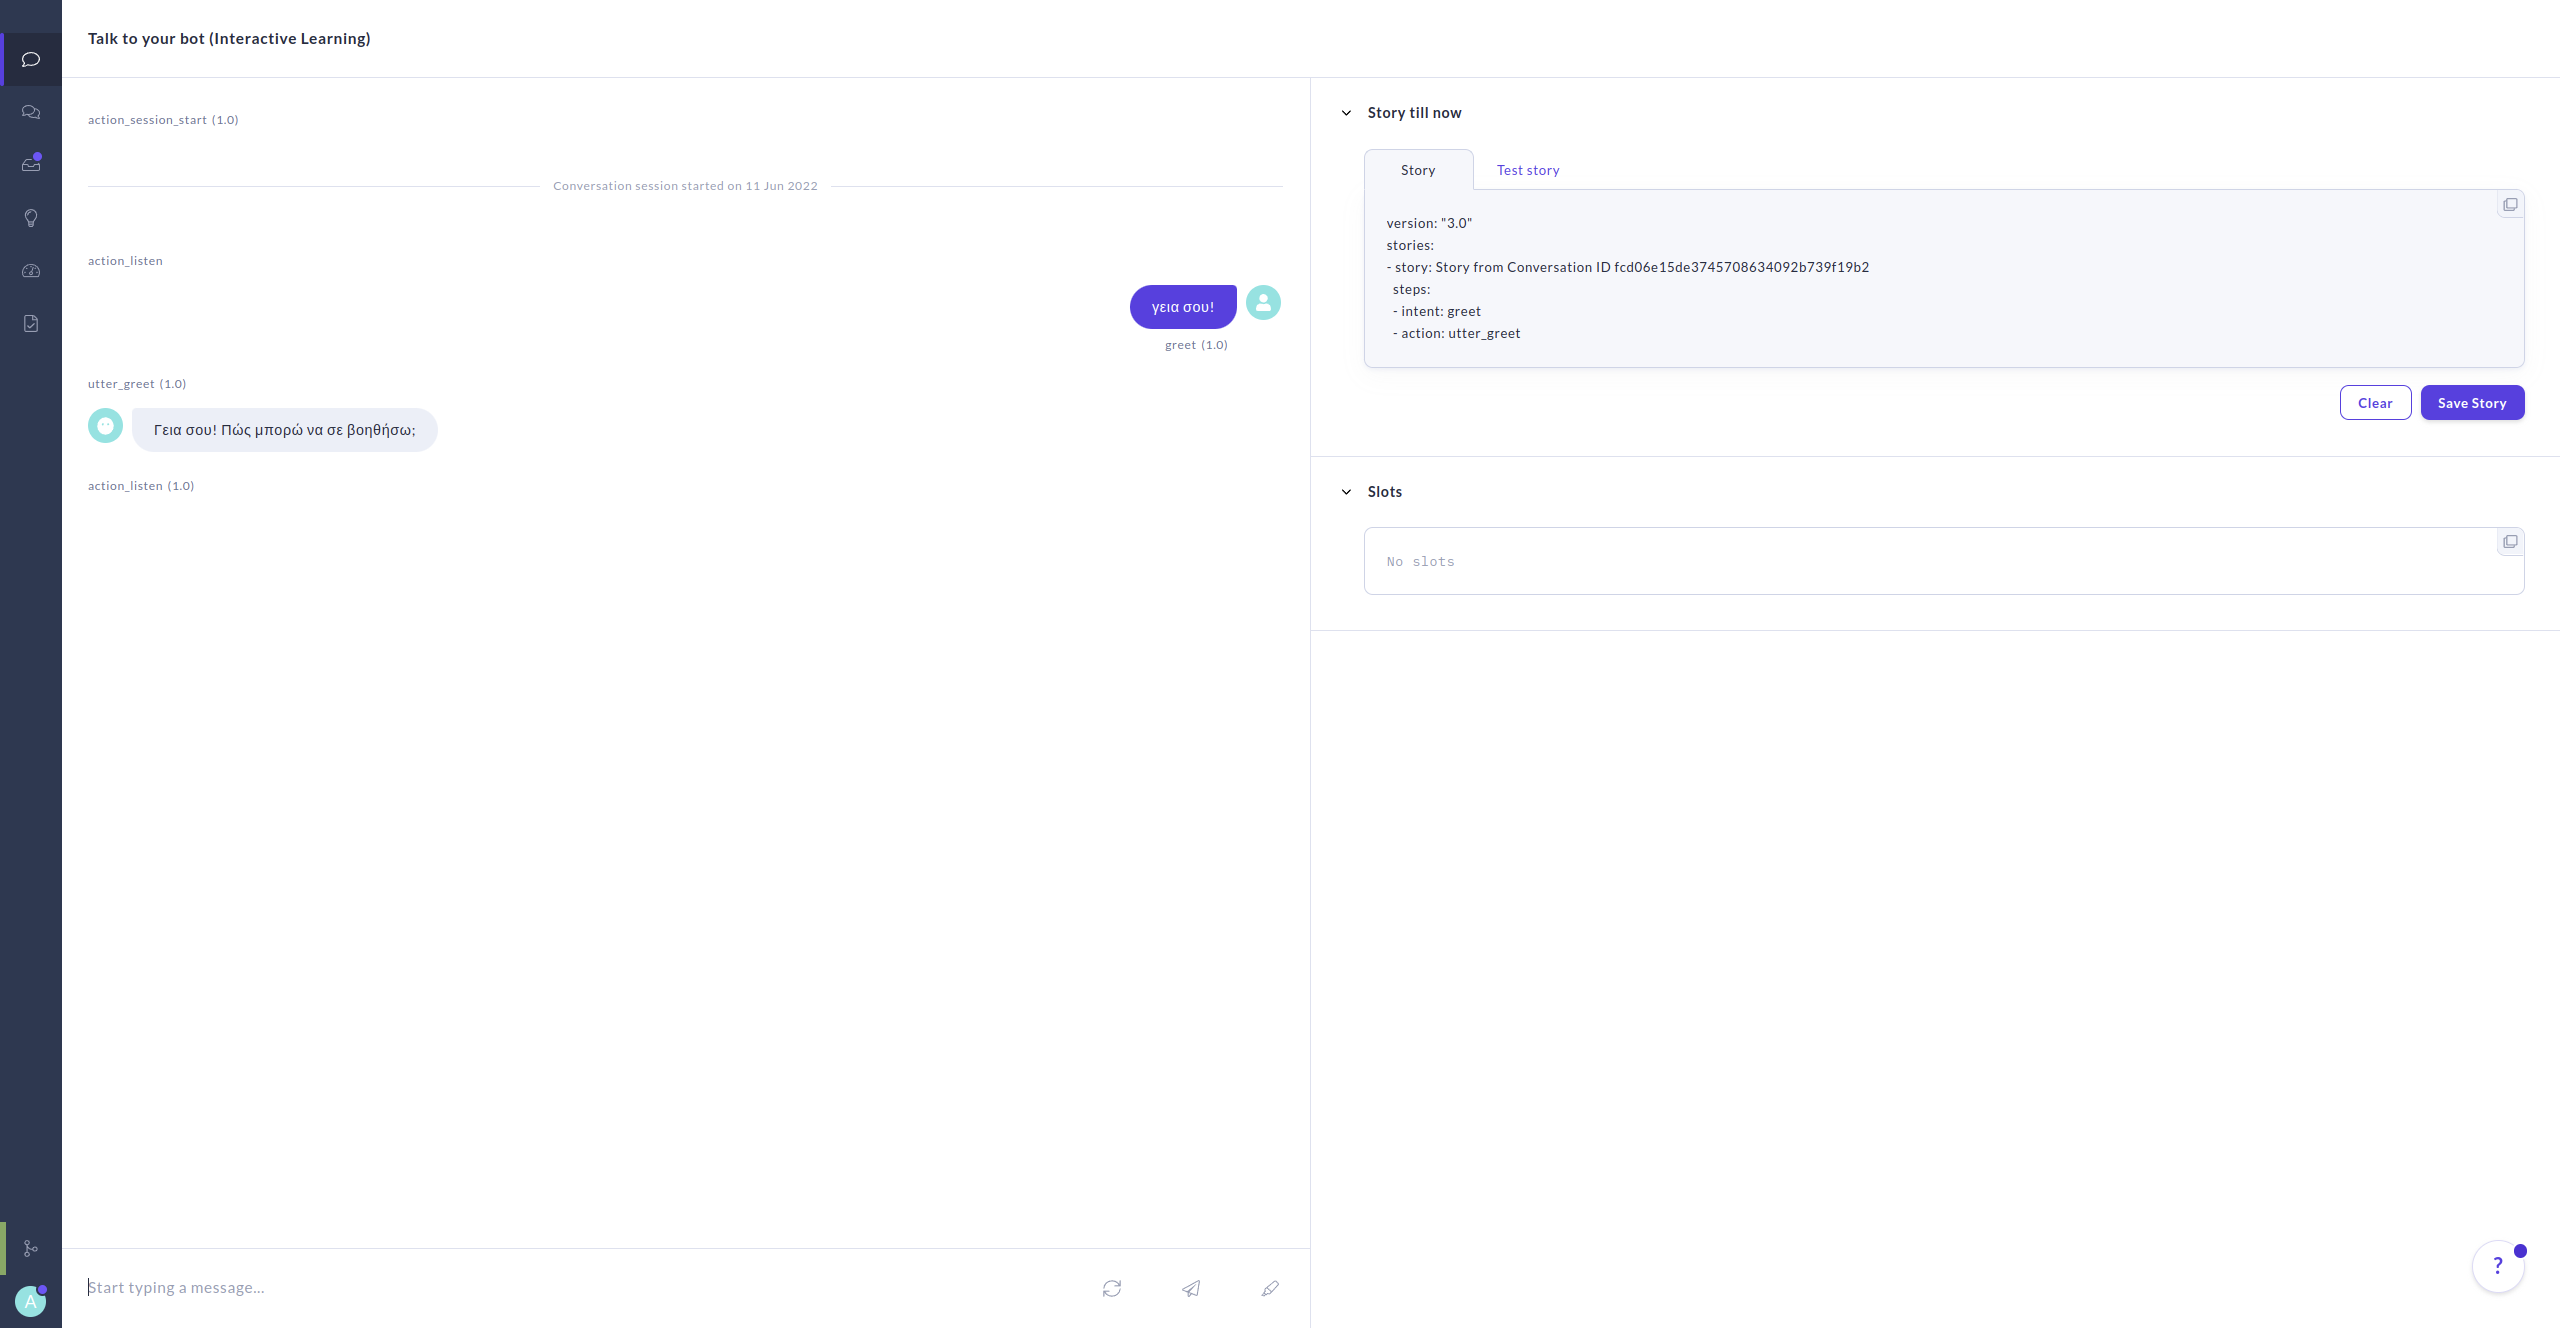
\includegraphics[width=1\textwidth]{images/appendix/rasax-conversation-interactive.png}
  \caption{\emph{RASA-X} διαδραστική συζήτηση με τον ψηφιακό βοηθό}
  \label{fig:rasax-conversation-interactive}
\end{figure}
\noindent

\begin{figure}[!ht]
  \centering
  \captionsetup{justification=centering}
  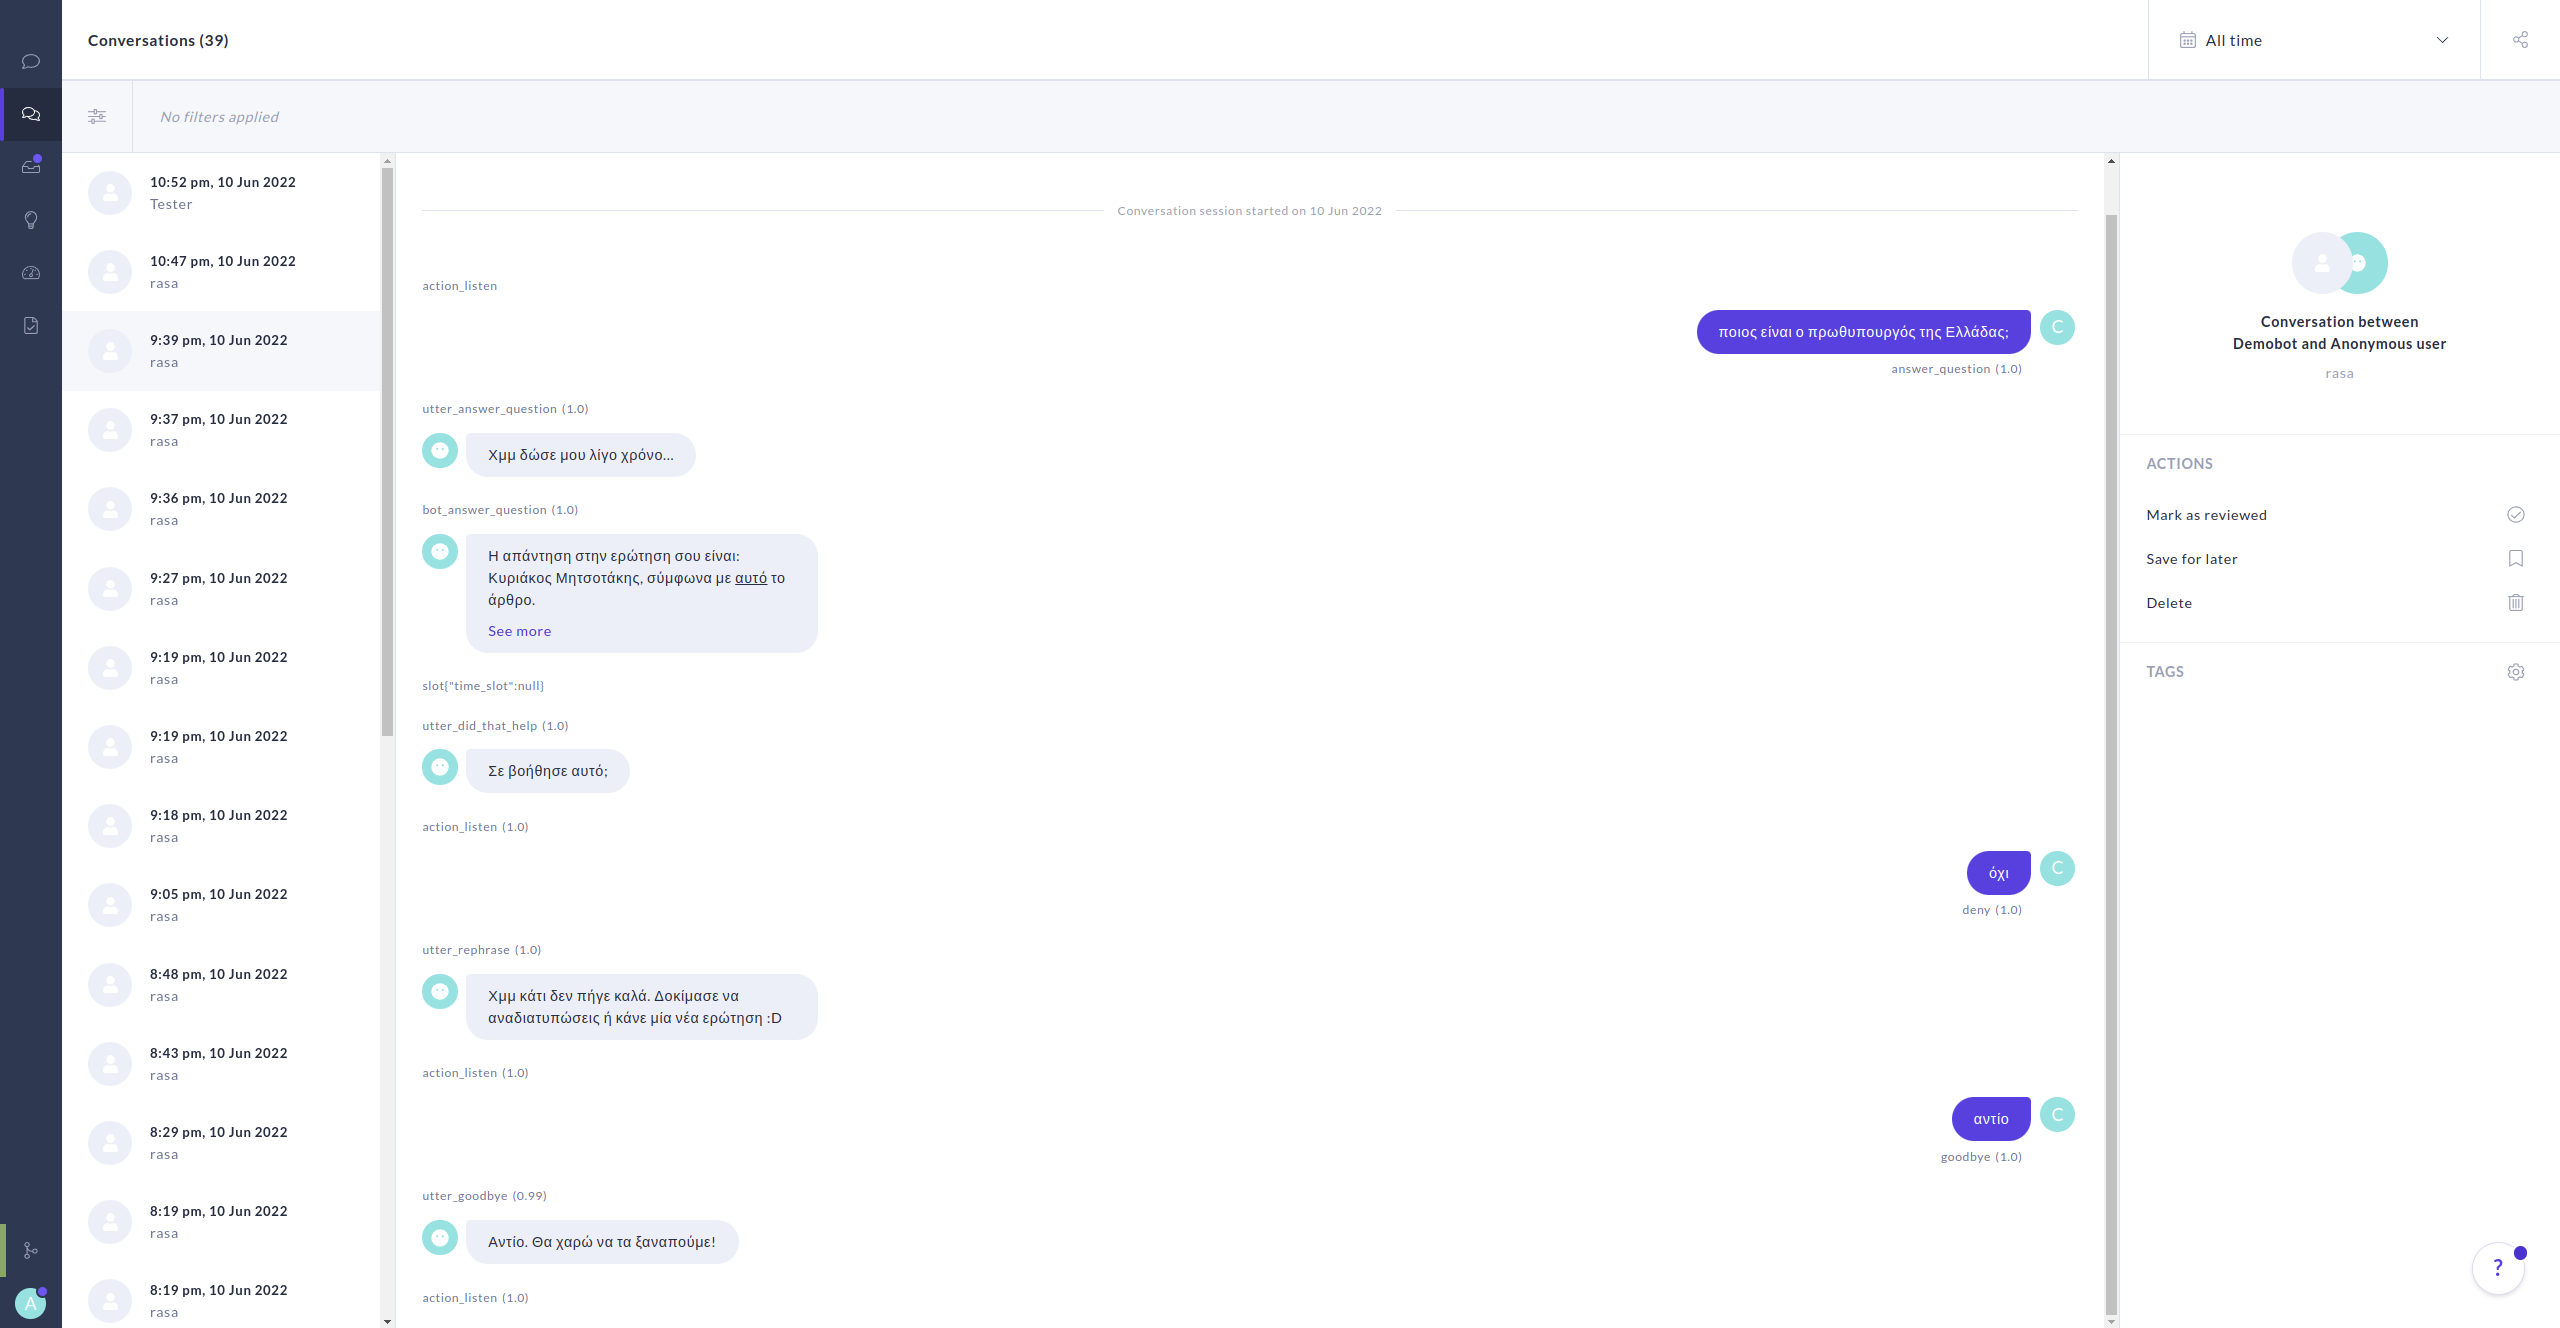
\includegraphics[width=1\textwidth]{images/appendix/rasax-conversation-review.png}
  \caption{\emph{RASA-X} αξιολόγηση υπάρχοντων συζητήσεων}
  \label{fig:rasax-conversation-review}
\end{figure}
\noindent